
\section{Minding the Gap}
\label{sec:evaluation}

We have established a necessary and sufficient condition for \cfreedom
that, if achievable, enables scalability limited to that of available
hardware: namely, server and network capacity. This raises two
important questions: what is the cost of not achieving the \cfree
condition, and how common is it? In this section, we begin to answer
both of these questions via both simple modeling and via a real-world,
proof-of-concept implementation of what is traditionally considered a
challenging OLTP benchmark. The former is the realm of traditional
concurrency control, while the latter is a first glimpse at what is
attainable via \cfree algorithms and their appropriate application
(Section~\ref{sec:futurework})

\subsection{Costs of Coordination}

When an application is \iconfluent and therefore executable with
\cfreedom, performance is largely uninteresting: there is no
fundamental reason why the application cannot attain indefinite
scalability. We will shortly quantify these benefits in a real-world
system, but, for now, we evaluate the alternative: what are the
scalability bottlenecks for non-\cfree applications?


\begin{figure}
\begin{center}
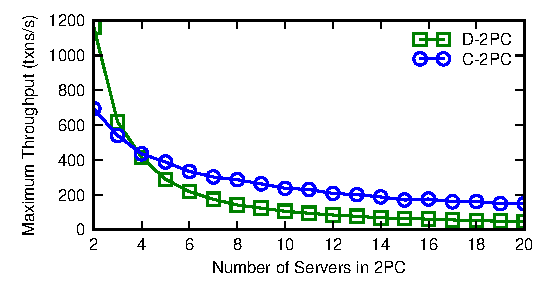
\includegraphics[width=\columnwidth]{figs/singledc-twopc.pdf}
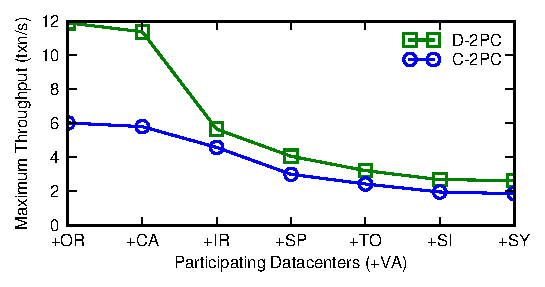
\includegraphics[width=\columnwidth]{figs/multidc-twopc.pdf}
\end{center}
\caption{Atomic committment as an upper bound on throughput over LAN
  and WAN.}
\label{fig:2pc}
\end{figure}

From traditional database systems, one of the primary challenges in
scaling database systems to both multiple replicas and across multiple
partitions is the atomic commitment problem: if a given transaction
can abort, all replicas (alternatively, partitions it accesses) must
agree to unilaterally commit or abort the transaction. This problem is
well-studied in both the database and distributed systems literature,
with many variants including two-phase commit, decentralized two-phase
commit, and three-phase commit. For each pair of conflicting
transactions, the servers responsible for the conflicting operations
must choose which (if either) should commit. This requirement for
mutual exclusion effectively means that the duration of atomic
commitment determines the maximum throughput for a given data item. If
atomic commit take $10$ms, then, for traditional algorithms, we can
achieve throughput of $100$ transactions per second per item. Indeed,
there are many possible optimizations we can exploit, including
batching and reordering of commits. Moreover, given non-conflicting
transactions, aggregate system throughput can be much higher than the
per-item throughput limitations. However, for arbitrary schedules of
transactions, atomic commitment latency is a reasonable upper bound on
throughput.

To better understand the relationship between atomic commitment
(necessitated by non-\iconfluent operations) and scalability, we
performed a simple analysis of achievable throughput under several
recently reported communication delays. We simulated the latency of
both traditional two-phase commit (three message delays with $3N$
messages) and decentralized two-phase commit (two message delays with
$N^2+N$ messages) under recently reported public cloud network delays
for null RPC or ping times. To improve performance, we do not simulate
local processing delays due to, say, locking, latching, or disk
delays: all overhead is due solely to coordination.

Figures 3A and 3B show our results for both local-area and wide-area
latencies.  In the local area, with only two servers participating in
atomic commitment (e.g., replication factor of $2$ or, alternatively,
two conflicting operations on items residing on different servers), we
see a maximum attainable throughput of around $600$ transactions per
second. With ten servers participating, throughput drops to only $200$
transactions per second: the long-tail of network latency surfaces as
the number of messages sent increases. In the wide area, the effects
are even more stark: if only coordinating within the continental US
from Virginia to Oregon, message delays incur a latency of around
$200$ milliseconds per commit: this results in a throughput of $5$
operations per second. If coordinating between all eight EC2
availability zones, throughput is only around $1$ transaction per
second.

While this study is based solely on reported latencies, deployment
systems corroborate our findings. For example, Google's F1 uses
optimistic concurrency control via WAN with commit latencies of
50-150ms. As the authors discuss, this limits throughput to between
$6-20$ transactions per second per item. Megastore's average write
latencies of $100-400$ms suggest similar throughputs to those that we
have predicted. Indeed, \textit{aggregate throughput} may be
substantially greater as multiple 2PC rounds for disjoint sets of data
items may safely proceed in parallel. However, \textit{worst-case}
access patterns will indeed greatly limit scalability: as many before
us have noted, adding more active servers/replicas in non-\cfree
models like serializability can greatly reduce throughput.

\subsection{Proof of Concept}

As a proof of concept application of \cfreedom analysis, we show that
the classic benchmark for OLTP performance is, indeed, not
particularly challenging from a concurrency control perspective. The
TPC-C benchmark is often used as the gold standard for database
concurrency control both in research and in industry, and in recent
years (despite the introduction of the TPC-E benchmark, whose
leaderboard is missing the current TPC-C world champion, Oracle) has
been used as a yardstick for distributed database performance (e.g.,
Calvin, H-Store, Silo). Accordingly, we determine the fundamental
scalability limitations of the backbone of this benchmark, the
New-Order transaction.

New-Order corresponds to the placement of an order in a wholesale
supplier application. Each new order randomly chooses a set of items,
decrements their stock, and records the order request in a designated
table. There are three challenging components of New-Order, which we
describe below:
\begin{itemize}

\item \textit{Foreign key constraints (Consistency Criteria
  3.3.2.4-7).} New-Order requires maintaining foreign key constraints:
  when an order is recorded in the \texttt{ORDER} table, the
  corresponding orders for each item should be reflected in the
  \texttt{ORDER-LINE} table. Similarly, the new order in the
  \texttt{ORDER} table should be present in the \texttt{NEW-ORDER}
  table. In a traditional database system, we might use locks to
  atomically control the visibility of these updates to multiple
  tables. However, our analysis of \lang tells us that we can maintain
  these constraints under insert with \cfreedom. Indeed, with the
  newly proposed \cfree RAMP algorithm, we can ensure that all of
  these updates are visible, or none are.

\item \textit{Sequential ID assignment (Consistency Criteria
  3.3.2.2-3).} Each New-Order executed in a pre-determined warehouse
  district should have a sequentially assigned ID (e.g.,
  \texttt{AUTO\_INCREMENT}). This poses a challenge: the
  \texttt{DISTRICT\_NEXT\_O\_ID} column must be incremented at the
  same time that corresponding rows are inserted into the
  \texttt{ORDER}, \texttt{NEW-ORDER}, and \texttt{ORDER-LINE}
  tables. We know from our analysis of \lang that this sequential
  assignment is not \cfree, so, for a compliant run, we will need to
  coordinate (note that others forego this sequential constraint CITE
  SILO at the expense of compliance). A naive approach would hold
  locks for the duration of each New-Order, but this greatly reduces
  throughput. Instead, we know that assigning a sequential ID cannot
  abort, so we simply wait to assign an order ID until commit. When
  inserting rows into the \texttt{ORDER}, \texttt{NEW-ORDER}, and
  \texttt{ORDER-LINE} tables, we assign a temporary key and, upon
  commit, rewrite this temporary key to point to the true sequential
  key. Accordingly, we only hold locks for a single atomic
  increment. Figure XX shows this process.

\item \textit{Maintaining stock levels.} When an order for a given
  item is placed, the stock for the given item must be adjusted
  accordingly. New-Order automatically replenishes the stock for a
  given item when it would otherwise become negative. Although not
  required by the benchmark, we can use a commutative \textit{counter}
  datatype to ensure that the final stock reflects all removals and
  additions to the stock as concurrent updates are made to a given item.
\end{itemize}

In all, TPC-C New-Order coordination can be limited to a single,
atomic increment-and-get operation on each district's order table. Our
\cfreedom analysis shows that all required constraints except one are
achievable without synchronous coordination. Hence, scalability---even
for a single warehouse---is limited to increment-and-get on a single
machine: several million transactions per second on modern
hardware. In contrast, the highest compliant TPC-C that respects this
sequential assignment is around $500,000$ New-Order transactions per
second (Oracle 11G). Compliant TPC-C results require scaling dataset
size with throughput, so contention is constant regardless of
throughput. However, the best known results in the research literature
that disregard this scaling are Calvin (500,000 serializable
transactions per second on 100 machines) and Silo (400,000
serializable transactions per second on 1 machine for sequential
IDs---which become the scaling bottleneck---and over 700,000
transactions per second for non-sequential IDs).

\begin{figure}
\begin{center}
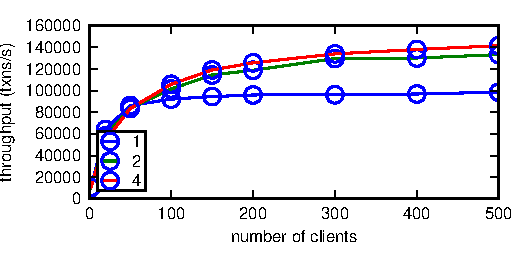
\includegraphics[width=\columnwidth]{figs/wh_thru.pdf}
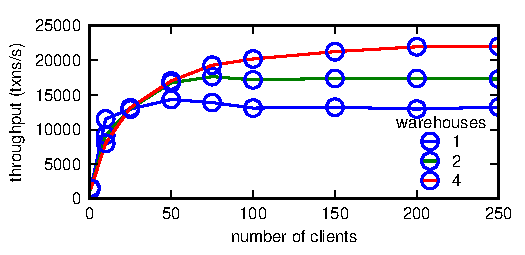
\includegraphics[width=\columnwidth]{figs/wh_thru_single.pdf}
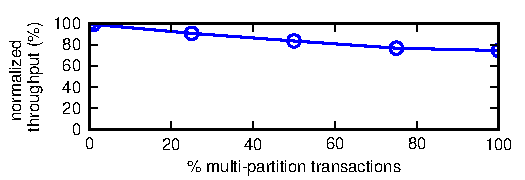
\includegraphics[width=\columnwidth]{figs/pct_thru.pdf}
\end{center}
\caption{Performance versus number of concurrent clients.}
\label{fig:clients}
\end{figure}


Unsurprisingly, as Figure YY shows, when we evaluate TPC-C New-Order
scaling on an in-memory database prototype, we can scale throughput
linearly to up to 100 machines. Distributed transactions do not affect
throughput except insofar as they consume additional CPU for
serialization and messaging. On a cluster of 100 EC2 cc2.8xlarge
instances spanning three us-west availability zones, we achieve over
1.8 million New-Order transactions per second. Contention is
negligible and, in our Java prototype, corresponds to a single
java.util.concurrent AtomicLong incrementAndGet() for each
transaction. Rather, each server is CPU bound due to our current,
fairly inefficient implementation: we achieve only 18,000
transactions/s/server on admittedly very powerful
hardware. Nonetheless, in a scale-out system, single-node performance
tuning is dwarfed by the power of largely-\cfree operations.

\begin{figure}
\begin{center}
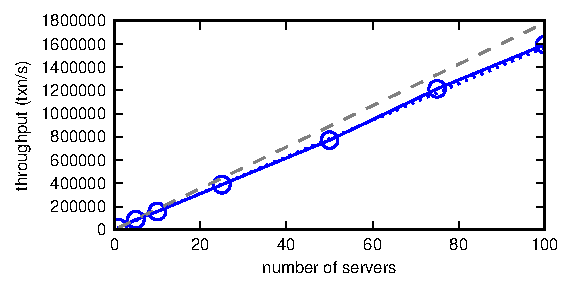
\includegraphics[width=\columnwidth]{figs/thru_scale.pdf}\vspace{-2em}
\end{center}
\caption{Scalability of TPC-C New-Order.}
\label{fig:clients}
\end{figure}


As Bailis et al. note, the remainder of the TPC-C transactions are
largely uninteresting from a concurrency control perspective. All
except for the Delivery transaction are implementable via a
combination of foreign key updates and commutative counter
increment/decrement, and the Delivery transaction is easily
implemented (as acknowledged in the benchmark specification) as a
single-partition transaction. The three (!)  consistency conditions in
the newer TPC-E benchmark represent a subset of the twelve conditions
from TPC-C that we consider here. Indeed, for the future, we are
proposing a more challenging benchmark designed to actually stress
concurrency control systems.
